%%%%%%%%%%%%%%%%%%%%%%%%%%%%%%%%%%%%%%%%%
% Masters/Doctoral Thesis 
% LaTeX Template
% Version 2.4 (22/11/16)
%
% This template has been downloaded from:
% http://www.LaTeXTemplates.com
%
% Version 2.x major modifications by:
% Vel (vel@latextemplates.com)
%
% This template is based on a template by:
% Steve Gunn (http://users.ecs.soton.ac.uk/srg/softwaretools/document/templates/)
% Sunil Patel (http://www.sunilpatel.co.uk/thesis-template/)
%
% Template license:
% CC BY-NC-SA 3.0 (http://creativecommons.org/licenses/by-nc-sa/3.0/)
%
%%%%%%%%%%%%%%%%%%%%%%%%%%%%%%%%%%%%%%%%%

%----------------------------------------------------------------------------------------
%	PACKAGES AND OTHER DOCUMENT CONFIGURATIONS
%----------------------------------------------------------------------------------------

\documentclass[
12pt, % The default document font size, options: 10pt, 11pt, 12pt
%oneside, % Two side (alternating margins) for binding by default, uncomment to switch to one side
english, % ngerman for German
singlespacing, % Single line spacing, alternatives: onehalfspacing or doublespacing
%draft, % Uncomment to enable draft mode (no pictures, no links, overfull hboxes indicated)
%nolistspacing, % If the document is onehalfspacing or doublespacing, uncomment this to set spacing in lists to single
%liststotoc, % Uncomment to add the list of figures/tables/etc to the table of contents
%toctotoc, % Uncomment to add the main table of contents to the table of contents
%parskip, % Uncomment to add space between paragraphs
%nohyperref, % Uncomment to not load the hyperref package
headsepline, % Uncomment to get a line under the header
%chapterinoneline, % Uncomment to place the chapter title next to the number on one line
%consistentlayout, % Uncomment to change the layout of the declaration, abstract and acknowledgements pages to match the default layout
]{MastersDoctoralThesis} % The class file specifying the document structure

\usepackage[utf8]{inputenc} % Required for inputting international characters
\usepackage[T1]{fontenc} % Output font encoding for international characters

\usepackage{mathptmx} % Use the Palatino font by default
\usepackage[]{algorithm2e}
\usepackage{amssymb}
\usepackage[backend=bibtex,style=numeric]{biblatex} % Use the bibtex backend with the authoryear citation style (which resembles APA)

\addbibresource{bibli.bib} % The filename of the bibliography

\usepackage[autostyle=true]{csquotes} % Required to generate language-dependent quotes in the bibliography

%----------------------------------------------------------------------------------------
%	MARGIN SETTINGS
%----------------------------------------------------------------------------------------

\geometry{
	paper=a4paper, % Change to letterpaper for US letter
	inner=2.5cm, % Inner margin
	outer=3.8cm, % Outer margin
	bindingoffset=.5cm, % Binding offset
	top=1.5cm, % Top margin
	bottom=1.5cm, % Bottom margin
	%showframe, % Uncomment to show how the type block is set on the page
}

%----------------------------------------------------------------------------------------
%	THESIS INFORMATION
%----------------------------------------------------------------------------------------

\thesistitle{Bayesian Network} % Your thesis title, this is used in the title and abstract, print it elsewhere with \ttitle
\supervisor{Dr. James \textsc{Smith}} % Your supervisor's name, this is used in the title page, print it elsewhere with \supname
\examiner{} % Your examiner's name, this is not currently used anywhere in the template, print it elsewhere with \examname
\degree{Doctor of Philosophy} % Your degree name, this is used in the title page and abstract, print it elsewhere with \degreename
\author{Sergiu \textsc{Breban}
Răzvan \textsc{Sălăjan}} % Your name, this is used in the title page and abstract, print it elsewhere with \authorname
\addresses{} % Your address, this is not currently used anywhere in the template, print it elsewhere with \addressname

\subject{Data Mining} % Your subject area, this is not currently used anywhere in the template, print it elsewhere with \subjectname
\keywords{} % Keywords for your thesis, this is not currently used anywhere in the template, print it elsewhere with \keywordnames
\university{Babes-Bolyai University} % Your university's name and URL, this is used in the title page and abstract, print it elsewhere with \univname
%\department{\href{http://department.university.com}{Department or School Name}} % Your department's name and URL, this is used in the title page and abstract, print it elsewhere with \deptname
%\group{\href{http://researchgroup.university.com}{Research Group Name}} % Your research group's name and URL, this is used in the title page, print it elsewhere with \groupname
\faculty{\href{http://www.cs.ubbcluj.ro/}{Facultatea de Matematică și Inforamtică}} % Your faculty's name and URL, this is used in the title page and abstract, print it elsewhere with \facname

\AtBeginDocument{
\hypersetup{pdftitle=\ttitle} % Set the PDF's title to your title
\hypersetup{pdfauthor=\authorname} % Set the PDF's author to your name
\hypersetup{pdfkeywords=\keywordnames} % Set the PDF's keywords to your keywords
}

\begin{document}

\frontmatter % Use roman page numbering style (i, ii, iii, iv...) for the pre-content pages

\pagestyle{plain} % Default to the plain heading style until the thesis style is called for the body content

%----------------------------------------------------------------------------------------
%	TITLE PAGE
%----------------------------------------------------------------------------------------

\begin{titlepage}
\begin{center}

\vspace*{.06\textheight}
{\scshape\LARGE \univname\par\facname}\vspace{1.5cm} % Babes-Bolyai University
% \textsc{\Large Doctoral Thesis}\\[0.5cm] % Thesis type

\HRule \\[0.4cm] % Horizontal line
{\huge \bfseries \ttitle\par}\vspace{0.4cm} % Thesis title
\HRule \\[1.5cm] % Horizontal line
 
\begin{minipage}[t]{0.8\textwidth}
\begin{flushleft} \large
\emph{Authors:}\\
{\authorname} % Author name - remove the \href bracket to remove the link
\end{flushleft}
\end{minipage}
% \begin{minipage}[t]{0.4\textwidth}
% \begin{flushright} \large
% % \emph{Supervisor:} \\
% % \href{http://www.jamessmith.com}{\supname} % Supervisor name - remove the \href bracket to remove the link  
% \end{flushright}
% \end{minipage}\\[3cm]
 
\vfill

%\large \textit{A thesis submitted in fulfillment of the requirements\\ for the degree of \degreename}\\[0.3cm] % University requirement text
%\textit{in the}\\[0.4cm]
%\groupname\\\deptname\\[2cm] % Research group name and department name
 
\vfill

{\large \today}\\[4cm] % Date
%\includegraphics{Logo} % University/department logo - uncomment to place it
 
\vfill
\end{center}
\end{titlepage}

%----------------------------------------------------------------------------------------
%	LIST OF CONTENTS/FIGURES/TABLES PAGES
%----------------------------------------------------------------------------------------
\begingroup
\let\cleardoublepage\clearpage
\tableofcontents
\endgroup

% \tableofcontents % Prints the main table of contents
\begingroup
\let\cleardoublepage\clearpage
\listoffigures % Prints the list of figures
\endgroup

\let\cleardoublepage\clearpage

%----------------------------------------------------------------------------------------
%	THESIS CONTENT - CHAPTERS
%----------------------------------------------------------------------------------------

\mainmatter % Begin numeric (1,2,3...) page numbering

\pagestyle{thesis} % Return the page headers back to the "thesis" style

% Include the chapters of the thesis as separate files from the Chapters folder
% Uncomment the lines as you write the chapters

% Chapter Template

\chapter{Data Mining} % Main chapter title

\label{Chapter1} % Change X to a consecutive number; for referencing this chapter elsewhere, use \ref{ChapterX}

%----------------------------------------------------------------------------------------
%	SECTION 1
%----------------------------------------------------------------------------------------

%-----------------------------------
%	SUBSECTION 1
%-----------------------------------
\section{Informatia inseamna putere}
In ziua de azi, datorita serviciilor ieftine de stocare a datelor, stocarea de informatii devine o treaba usoara si deschide calea invatarii unor lucruri noi. Asadar obtinerea de noi cunostine se transforma in serviciul de extragere prin diferite metode de noi idei  dintr-un ocean de informatii stocate care asteapta sa fie analizate. In zilele noastre majoritea actiunilor cotidiene sunt inregistrate si stocate. Datorita numarului mare de oameni si de actiuni pe care un om le face se transmit date intr-un volum greu de imaginat. Avand disponibil un volum atat de imens de date partea mai grea devine analiza, invatarea si corelarea acestora. Desi lucrul cu date a fost folosit de mult timp de catre economisti, statisticieni sau meteorologi e de remarcat cresterea recenta al oportunitatilor de gasire al modelelor in date. Bazat pe \cite{DMP2011} numarul datelor la nivel global stocat in bazele de date se dubleaza la fiecare 20 de luni. Avand in vedere volumul imens de date cu care suntem inundati si eficientizarea calculatoarelor de a suporta cautari are ca urmare cresterea interesului in data mining. Astfel, data mining, reprezinta o solutie la a gasi noi concepte, noi idei care pot ajuta la rezolvarea unor probleme din diferite ramuri, de exemplu, intr-un context comercial, obtinandu-se un avantaj comercial. 

%-----------------------------------
%	SUBSECTION 2
%-----------------------------------
\section{Definitie}
Data mining reprezinta procesul de analiza si cercetare asupra unui volum imens de date stocat in baze de date sau alte tipuri de stocare de informatii. Procesul are ca scop descoperirea de noi cunostinte precum: modele, asocieri, comportamente, anomalii, structuri semnificative care sa ofere descoperiri noi, inovatoare. Procesul poate fi privit ca o cutie inchisa care produce rezultatul dorit. La fel cum si \cite{Disco} precizeaza, procesul de data mining poate avea si rezultate nedorite daca o metoda este aplicata intr-un context nepotrivit sau modelele sunt construite pe presupuneri eronate.   

%-----------------------------------
%	SUBSECTION 3
%-----------------------------------
\section{CISP}
"Cross-industry standard practice"(CISP) reprezinta un proces standard de abordare al solutiilor de tip data mining. Acest standard a fost creat cu scopul de a fi liber si de a fi utilizat de catre toti cei care folosesc data mining pentru a rezolva diferite probleme. A fost creat, cumva natural, datorita faptului ca fiecare incerca sa isi fac propriul proces, astfel creandu-se haos. Asadar, CISP, a luat nastere ca fiind un standard care nu e specific unei industrii, aplicatii, sau unui tool. Bazat pe standardul CISP, un proiect de tip data mining consta din 6 etape dupa cum se poate vedea si din Figure~\ref{fig:CISP}. 
\begin{figure}[th]
\centering
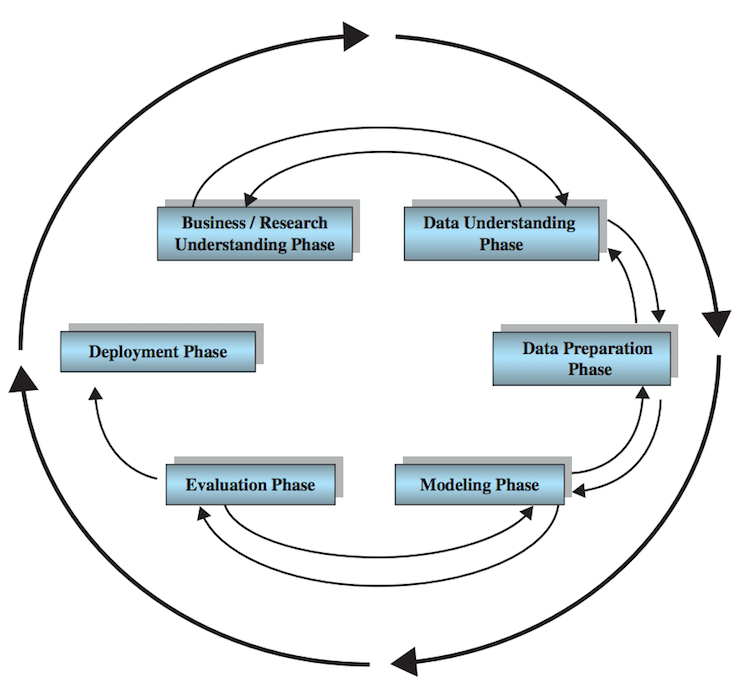
\includegraphics{Figures/CISP}
\decoRule
\caption[CISP]{CISP}
\label{fig:CISP}
\end{figure}
Procesul definit e unul iterativ care se poate adapta; fiecare componenta depinde de componenta precedenta iar in caz de iregularitati procesul se poate intoarce inapoi la pasul precedent.
% %-----------------------------------
% %	SUBSECTION 3_1
% %-----------------------------------
% \subsection{CISP}

%Data mining poate fi asociat cu expresii precum descoperirea de cunostinte in baze de date, (potrivit lui \cite{JiaweiIntro}), cu toate ca alti cercetatoti considera, data mining, ca fiind un pas important in descopeirirea de noi cunostinte. Se poate sintetiza procesul de descoperire a cunostintile din date in urmatorii pasi (bazat pe \cite{JiaweiIntro}): curatarea datelor, integrarea datelor, selectarea datelor, transformarea datelor, extragerea datelor, evaluarea modelelor si prezentarea cunostintelor. Acesti 7 pasi pot fi impartiti in 2 grupuri mai mari. Primii 4 pasi pot fi priviti ca construirea unor depozite de date si efectuare unor operatii pe acestea. Ultimii 3 pasi se transforma intr-un proces iterativ denumit data mining.  

%-----------------------------------
%	SUBSECTION 4
%-----------------------------------
\section{La ce se foloseste?}

Cerintele in care data mining e folosit s-au grupat in 6 clase (potrivit cu \cite{Disco}).
\begin{itemize}
\item Descrierea: reprezinta modul prin care se cauta cai care precizeaza unele "trenduri" sau modele care se observa in date.
\item Estimarea: se refera la a estima valoarea numerica a unui atribut tinta avand la dispozitie variabile predictorii care pot fi de tipul numerice sau categoriale(?). De exemplu se pot face estimari despre cat v-a cheltui o familie cu 2 copii pentru inceperea unui nou an scolar. De asemenea, un alt exemplu il reprezinta prezenta la vot pentru alegerile curente ale cetatenilor cu varsta cuprinsa intre [18-24] cu drept de vot bazat pe alegerile din anii trecuti.
\item Predictia: este similara cu estimarea si clasificarea cu precizarea ca rezultatul predictiei o sa se intample in viitor. Exemple de predictii ar fi: pretul unei actiuni la bursa peste cateva luni sau cine va castiga campionatul mondial de fotbal. Bazat pe \cite{Disco}, in alegerile prezidentiale din America din 2012, echipa de campanie a lui Barack Obama s-a folosit de data mining. Acestia au folosit data mining pentru a identifica tipul sustinatorilor lui Barack Obama si s-au asigurat ca acestia merg la vot si au mai folosit pentru a face predictii despre voturile pentru Barack Obama in fiecare judet. Un exemplu de predictie pentru judetul Hamilton din statul Ohio considerat "indecis", a fost de 56.4\% iar rezulultul final a fost de 56.6\%.
\item Clasificarea: este asemantoare cu estimarea cu diferenta ca variabila tinta, care se doreste sa fie clasificata, are ca valori categorii. Modelul de data mining examineaza datele care contini valori pentru atributele predictorii si atributul tinta.
\item Gruparea: se refera la procesul de a grupa date, observatii, cazuri in clase asemanatoare. O grupare reprezinta o colectie de obiecte care prezinta insusiri asemanatoare intre ele. Gruparea reprezinta o sarcina diferita conceptual fata de clasificare, estimare sau predictia. In procesul de grupare nu exista un atribut tinta care sa fie clasificat. In schimb, gruparea, incearca sa imparta datele in grupuri sau clase relativ omogene, astfel incat similaritatiile elementelor dintr-un grup sunt maximizate iar disimilaritatille cu elemente straine grupului sunt minimizate.
\item Asocierea: consta in a determina ce atribute "merg impreuna". Are ca scop gasirea de legaturi intre atribute. Este folosita cu succes in analiza pietei cumparatorilor din magazine pentru a gasi ce produse sunt cumparate impreuna si ce produce nu sunt. Asocierile sunt de forma "daca antecedentul atunci consecinta".
\end{itemize}

% Chapter Template

\chapter{Rețeaua Bayesiană} % Main chapter title

\label{Chapter2} % Change X to a consecutive number; for referencing this chapter elsewhere, use \ref{ChapterX}

%-----------------------------------
%	SECTION 1
%-----------------------------------
\section{Definiție}

O rețea Bayesiană este un model probabilistic grafic care reprezintă un set de variabile aleatoare și dependețele condiționale dintre ele sub forma unui graf orientat aciclic (DAG).

Fiecare nod al grafului reprezintă o variabilă aleatoare, iar arcele dintre noduri reprezintă dependențele probabilistice dintre nodurile conectate.

Clasificatorul naiv Bayes presupune că toate variabilele sunt independent condiționate, în contrast cu rețelele Bayesiene, care permite condiționarea independentă aplicată la subseturi de variabile.

Aceste modele probabilistice, ca modelul naiv Bayes sau modelele logistice de regresie sunt diferite de alte modele de reprezentare, cum ar fi arborii de decizie, prin faptul că produc estimări probabilistice în loc de clasificări exacte.

Pentru fiecare clasă de valori, estimează probabilitatea ca o instanță dată să aparțină acelei clase.
Aceste estimări probabilistice sunt mai utile decât simple predicții, deoarece pot fi clasate, iar costul acestora poate fi minimizat.

%-----------------------------------
%	SECTION 2
%-----------------------------------
\section{Deducția rețelei Bayesiene}

Deducția rețelei Bayesiene se realizează în 3 pași:
\begin{itemize}
\item Deducția de variabile neobservate; rețeaua poate fi folosită pentru a oferi informații probabilistice despre relațiile dintre variabile.
\item Învățarea probabilităților condiționale; pentru fiecare nod specificarea distribuției probabilităților condiționate de părinții nodului respectiv.
\item Învățarea structurii rețelei și construirea grafului.
\end{itemize}

%-----------------------------------
%	SECTION 3
%-----------------------------------
\section{Învățarea rețelei Bayesiene}

Algoritmul pentru construirea rețelei Bayesiene are două componente: o funcție pentru evaluarea rețelei în funcție de date și o metodă de a genera toate rețelele posibile și a o selecta pe cea mai bună.

După definirea structurii grafului care reprezintă rețeaua, calculul probabilităților condiționale este ușor de realizat, necesitând doar calculul frecvențelor relative a combinațiilor de atribute asociate din setul de date.

\subsection{Teorema lui Bayes}

Pentru a putea exprima în termeni matematici teorema lui Bayes, se folosesc anumite  notaţii.  Considerăm  o  ipoteză  h  din  spaţiul  ipotezelor  H.  Prin  P(h)  notăm probabilitatea iniţială a ipotezei h. Prin P(D) ne referim la probabilitatea anterioară observării datelor de antrenare D, iar la probabilitatea de a observa datele D în raport cu ipoteza h, prin P(D|h).  Deşi  trebuie  să  avem  în  vedere  toate  acestea,  în  lumea  maşinilor  de  învăţare  suntem interesaţi de o altă probabilitate notată prin P(h|D). Aceasta este probabilitatea ulterioară a lui h, aceea ca ipoteza h să se petreacă având în vedere datele de antrenare D. Aceasta reflectă influenţa datelor de antrenare  asupra decizilor care pot fi luate, în contrast cu P(h), probabilitate independent de D.

Teoremalui  Bayes furnizează metoda de a calcula probabilitatea ulterioară, P(h|D), din P(h), P(D) şi P(D|h), astfel:
\[
	P(h|D)=\frac{P(D|h)*P(h)}{P(D)}
\]

% %-----------------------------------
% %	SECTION 4
% %-----------------------------------
\section{Reprezentarea datelor}

Pentru reprezentarea datelor, un format foarte răspândit este formatul ARFF, datele fiind stocate într-un fișier cu formatul .arff. Acest format permite definirea atributelor și a valorilor posibile pentru fiecare atribut, cât și un set de instanțe, cu valori specificate pentru fiecare atribut.

Exemplu de fișier .arff:\\
@relation skiing \\
@attribute temperature \{ hot, mild, cool \}\\
@attribute windy \{ true, false \}\\
@attribute outlook \{ sunny, overcast \}\\
@attribute snowCover \{ low, medium, high \}\\
@attribute rainfall \{ sleet, rain, snow, none \}\\
@attribute ski? \{ yes, no \}\\
@data\\
hot, false, overcast, medium, none, no\\
hot, true, sunny, high, none, no\\
hot, true, sunny, high, sleet, no\\
mild, false, sunny, high, none, yes\\
mild, false, sunny, low, none, no\\
cool, true, sunny, medium, none, yes\\
cool, true, overcast, medium, snow, no\\

Acest set de date reprezintă starea unei pârtii de ski, caracterizată de 5 atribute, cu valorile corespunzătoare:\\
temperature \{ hot, mild, cool \}\\
windy \{ true, false \}\\
outlook \{ sunny, overcast \}\\
snowCover \{ low, medium, high \}\\
rainfall \{ sleet, rain, snow, none \}\\

%-----------------------------------
%	SUBSECTION 4
%-----------------------------------
\section{Algoritm de învățare a structurii}

Odată reprezentate datele, avem nevoie de algoritmi specifici pentru a construi și inițializa structura rețelei Bayesiene.

Un exemplu de structură pentru setul de date despre starea pârtiei de ski poate fi observat în Figura ~\ref{fig:structure}.

\begin{figure}[th]
\centering
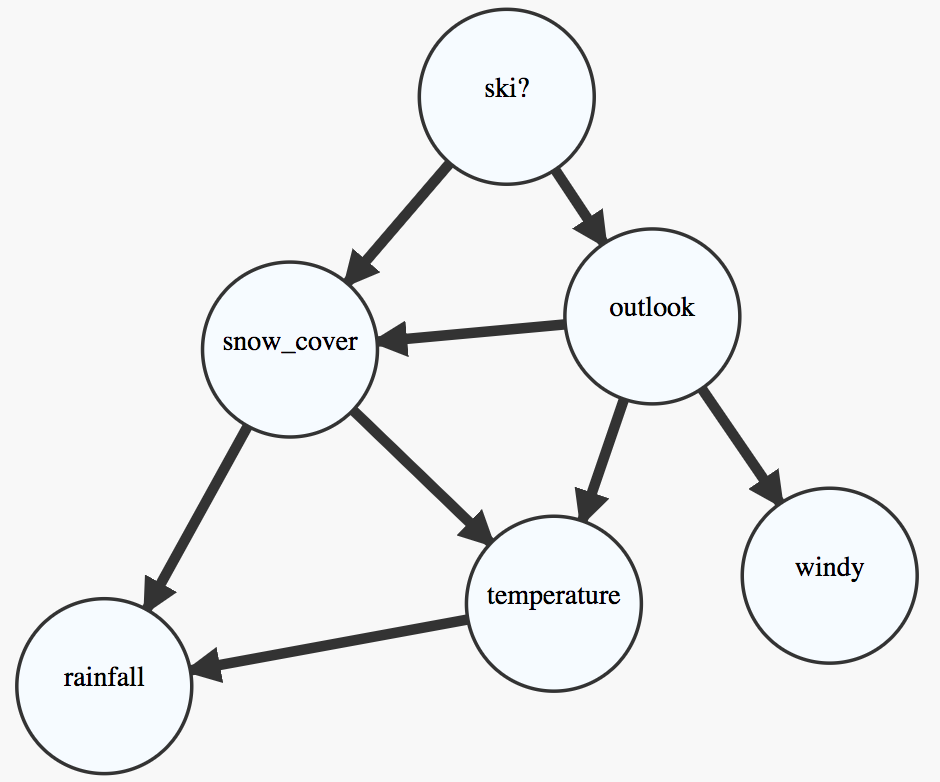
\includegraphics[scale=0.4]{Figures/structure}
\decoRule
\caption{Strucura unei rețele bayesiene}
\label{fig:structure}
\end{figure}

Unul dintre cei mai eficienți algoritmi pentru construirea structurii este algorimul K2, iar pentru calcul costului unui graf în cadrul algorimului de căutare, funcția de scor K2, propusă de Cooper and Herskovits (1992). \cite{carvalho2009scoring}

\subsection{Algoritmul K2}

Algoritmul K2 începe cu o ordine dată a atributelor (noduri) și încearcă să adauge o muchie de la nodurile procesate la cel curent, astfel încât scorul rețelei să fie maxim.

Numărul maxim de părinți poate fi restricționat pentru un nod (la 2 de exemplu) pentru a evita overfitting-ul. În funcția de scor K2 și în calcului tabelelor probabilităților condiționale se poate folosi estimatorul Laplace. \cite{ruiz2005illustration}

În continuare este prezentat algoritmul K2 \cite{cooper1992bayesian}, care caută cea mai probabilă structură a rețelei printr-o metodă euristică, fiind dat un set de cazuri D:

\begin{algorithm}[H]
	\KwData{Un set de n noduri, o ordine a nodurilor, o limită u a numărului de părinți pentru un nod și o bază de date D conținând m cazuri}
	\KwResult{Pentru fiecare nod, un set de părinți}
	\For{$i\leftarrow 1$ \KwTo $n$} {
		$\pi_i \leftarrow \emptyset$\;
		$P_{old} \leftarrow f(i, \pi_i)$ \{Această funcție este calculată folosind ecuația de mai jos\}\;
		$OKToProceed \leftarrow true$\;
		\While{OKToProceed and $|\pi_i| < u$} {
			let $z$ be the node in $Pred(x_i) - \pi_i$ that maximizes $f(i, \pi_i \cup \{z\})$\;
			$P_{new} \leftarrow f(i, \pi_i \cup \{z\})$\;
			\If{$P_{new} > P_{old}$} {
				$P_{old} \leftarrow P_{new}$\;
				$\pi_i \leftarrow \pi_i \cup \{z\}$\;
			}
			\Else {
				OKToPreceed $\leftarrow$ false\;
			}
		}
		write('Node: ', $x_i$, 'Parent of $x_i$: ', $\pi_i$)\;
	}
\end{algorithm}

Ecuația:
\[
	f(i, \pi_i) = \prod_{j=1}^{q_i} \frac{(r_i-1)!}{N_{ij}+r_i-1)!} \prod_{k=1}^{r_i} \alpha_{ijk}!
\]

Unde: \\
$\pi_i$ : setul de părinți pentru nodul $x_i$ \\
$q_i = |\phi_i|$ \\
$\phi_i$ : lista posibilelor instanțe de părinți pentru $x_i$ \\
$r_i = |V_i|$ \\
$V_i$ : lista tuturor valorilor posibile pentru atributul $x_i$ \\
$\alpha_{ijk}$ : numărul de cazuri în D în care atributul $x_i$ este instanțiat cu a $k$-a lui valoare, iar părinții lui $x_i$ în $\pi_i$ sunt instanțiați cu a $j$-a valoare în $\phi_i$ \\
$N_{ij} = \sum_{k=1}^{r_i} \alpha_{ijk}$ : numărul de instanțe din D unde părinții lui $x_i$ în $\pi_i$ sunt instanțiați cu a $j$-a valoare în $\phi_i$
 

%----------------------------------------------------------------------------------------
%	BIBLIOGRAPHY
%----------------------------------------------------------------------------------------
\begingroup
\let\cleardoublepage\clearpage
\printbibliography[heading=bibintoc]
\endgroup
%----------------------------------------------------------------------------------------

\end{document}  
